
\chapter{Method}

\section{Model description}
The model that is developed in this thesis consists of two parts. As a first step, Matrix Factorization is applied to make a first prediction on the missing drug target pairs. Matrix Factorization predicts the missing values based only on the observations in the training dataset and does not take additional features of the drugs and targets into account. This is where the second part of the model, Continuous Conditional Random Fields comes into play. The Continuous Conditional Random Field gets the similarity matrices of the drugs and targets as input, together with the training dataset and the predictions that were made by Matrix Factorization on the training dataset. The intuition behind the CCRF is then to first learn:
\begin{itemize}
\item how \textit{trust-worthy} the MF prediction is (based on the MF predictions that were made on the test data)
\item how similar in terms of binding behaviour, similar drugs and similar targets (similar meaning, high similarity values are given in the similarity matrices) are.
\end{itemize}

The \textit{trust-worthyness} of the MF prediction and the agreement of binding behaviour with similarity of the drugs/targets correspond to parameters $\alpha$ and $\beta$ in the formulation of the CCRF. With the learned parameters $\alpha$ and $\beta$ the CCRF predicts the missing values based on the MF predictions that were made on the missing values and by interpolating between similar drugs/targets. Details of both MF and the CCRF are given in the following sections. The main focus of the developed method in this thesis is on the CCRF part. The model is illustrated in Figure \ref{fig:pipeline} as a pipeline.

\begin{figure}
\begin{center}
  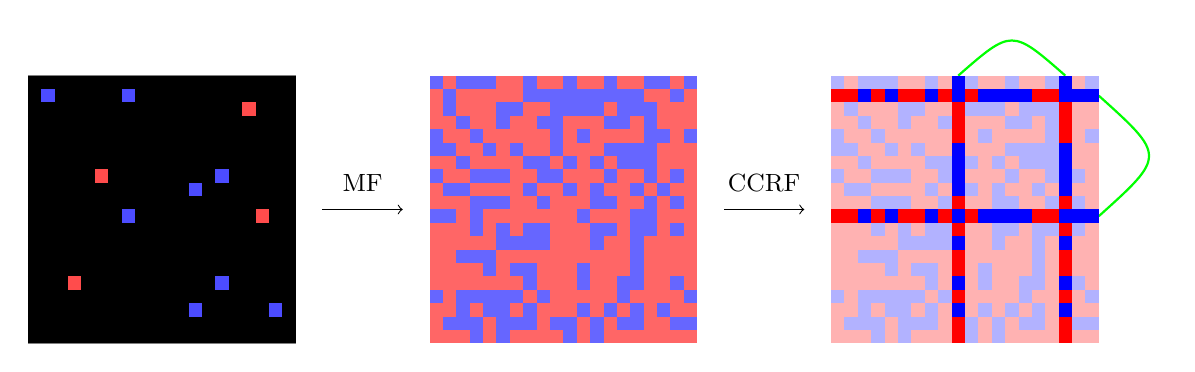
\begin{tikzpicture}[scale=0.17]
  
  \foreach \x in {0,...,19}
  	\foreach \y in {0,...,19}{
   	 \fill [red!60] (\x+30,\y) rectangle (\x+31,\y+1);
   	 \fill [red!30] (\x+60,\y) rectangle (\x+61,\y+1);
   	 }
   	 
   \foreach \x in {0,...,200}{
   	 \pgfmathsetmacro{\Xa}{random(19)}
   	 \pgfmathsetmacro{\Xb}{random(19)}
   	  \fill [blue!60] (\Xa+29,\Xb) rectangle (\Xa+30,\Xb+1);
   	  \fill [blue!60] (33,0) rectangle (34,1);
   	  \fill [blue!60] (35,0) rectangle (36,1);
   	  \fill [blue!60] (40,0) rectangle (41,1);
   	  \fill [blue!60] (42,0) rectangle (43,1);
   	  \fill [blue!60] (49,19) rectangle (50,20);
   	  \fill [blue!60] (49,15) rectangle (50,16);
   	  \fill [blue!60] (49,1) rectangle (50,2);
   	  \fill [blue!60] (49,3) rectangle (50,4);
   	  
   	  \fill [blue!30] (\Xa+59,\Xb) rectangle (\Xa+60,\Xb+1);
   	  \fill [blue!30] (63,0) rectangle (64,1);
   	  \fill [blue!30] (65,0) rectangle (66,1);
   	  \fill [blue!30] (70,0) rectangle (71,1);
   	  \fill [blue!30] (72,0) rectangle (73,1);
   	  \fill [blue!30] (79,19) rectangle (80,20);
   	  \fill [blue!30] (79,15) rectangle (80,16);
   	  \fill [blue!30] (79,1) rectangle (80,2);
   	  \fill [blue!30] (79,3) rectangle (80,4);
   	  }
   	  
   	  \draw [->] (22,10) to (28,10);
   	  
   	  \draw[help lines] (0,0) grid (20,20);
\fill [black] (0,0) rectangle (20,20);
\fill [red!70] (3,4) rectangle (4,5);
\fill [red!70] (5,12) rectangle (6,13);
\fill [blue!70] (14,12) rectangle (15,13);
\fill [red!70] (12,2) rectangle (13,3);
\fill [blue!70] (12,2) rectangle (13,3);
\fill [blue!70] (12,11) rectangle (13,12);
\fill [blue!70] (7,9) rectangle (8,10);
\fill [red!70] (17,9) rectangle (18,10);
\fill [blue!70] (7,18) rectangle (8,19);
\fill [blue!70] (1,18) rectangle (2,19);
\fill [blue!70] (18,2) rectangle (19,3);
\fill [blue!70] (14,4) rectangle (15,5);
\fill [red!70] (16,17) rectangle (17,18);

\draw [->] (52,10) to (58,10);

\draw [color=green, thick] (80,9.5) .. controls (85,14) .. (80,18.5);
\draw [color=green, thick] (69.5,20) .. controls (73.5,23.5) .. (77.5,20);
%\draw [color=green, thick] (62.5,20) .. controls (65.5,23.5) .. (68.5,20);
%\draw [color=green, thick] (80,2.5) .. controls (85,8.5) .. (80,14.5);

\foreach \x in {0,...,19}{
	\fill [red] (\x+60,18) rectangle (\x+61,19);
	\fill [red] (\x+60,9) rectangle (\x+61,10);
	%\fill [red] (\x+60,2) rectangle (\x+61,3);
	%\fill [red] (\x+60,14) rectangle (\x+61,15);
	\fill [red] (69,\x) rectangle (70,\x+1);
	\fill [red] (77,\x) rectangle (78,\x+1);
	%\fill [red] (62,\x) rectangle (63,\x+1);
	%\fill [red] (68,\x) rectangle (69,\x+1);
}
\foreach \x in {0,...,10}{
   	 \pgfmathsetmacro{\Xa}{random(19)}
   	 	\fill [blue] (\Xa+60,18) rectangle (\Xa+61,19);
   	 	\fill [blue] (\Xa+60,9) rectangle (\Xa+61,10);
   	 	
   	 	
   	 	\fill [blue] (69,\Xa) rectangle (70,\Xa+1);
   	 	\fill [blue] (77,\Xa) rectangle (78,\Xa+1);
   	}
   	
   	\node at(55,12){\small CCRF};
   	\node at(25,12){\small MF};
	\end{tikzpicture} 

	\end{center}
	\caption{First, Matrix Factorization is applied to get an initial prediction, then a graphical model (CCRF) is utilized to introduce similarity matrices of the drugs and targets.}
	\label{fig:pipeline}
	\end{figure}
\subsection{Matrix Factorization}

The Matrix Factorization technique has been demonstrated to be effective specially for personalized recommendation tasks \cite{Koren:2009:MFT:1608565.1608614} and it has been previously applied for drug target interaction prediction (\cite{liu2016neighborhood}, \cite{ezzat2016drug}, \cite{gonen2013kernelized}). In general, Matrix Factorization is a process in which a sparsely filled training matrix $R$ is approximated by the product of two factor matrices $P \in \mathbb{R}^{k\times m}$ and $Q \in \mathbb{R}^{k\times n}$. In the given problem, the given values in $R$ are the experimentally validated drug-target interaction strengths and the task is to predict the missing values in the matrix. With learned matrices $P$ and $Q$, a missing affinity of drug-target pair $(d_i, t_j)$ in $R$ can be predicted by the inner product of column $i$th of $P$ and the $j$th column of $Q$.
The factor matrices $P$ and $Q$ are learned by minimizing the regularized squared error on the set of known affinities:
\begin{center}
$\min\limits_{Q,P}{\sum\limits_{(d_i,t_j)\in \kappa} (a_{i,j}-q_i^Tp_j)^2} + \lambda (||p||^2 + ||q||^2)$
\end{center}
where $\kappa$ is the set of drug-target pairs $(d_i,t_j)$ for which the binding affinity is known. The above optimization problem can be solved by stochastic gradient descent as described in \cite{Koren:2009:MFT:1608565.1608614}.

For the experiments in this thesis the LIBMF package was used in R \cite{chin2016libmf}.

\subsection{Continuous Conditional Random Fields}

\subsubsection{Introduction to Conditional Random Fields}

Conditional Random Fields were originally developed for the task of segmenting and labeling sequence data \cite{lafferty2001conditional}. In contrast to predicting continuous values as for drug target binding affinities, the original formulation predicts a label vector $Y$, where all components of $Y_i$ are assumed to range over a finite label alphabet $\mathcal{Y}$. 

%(non-continuous) Conditional Random Fields were applied successfully for tasks, such as ...

To the best of my knowledge, the continuous variant of Conditional Random fields were first introduced by \cite{qin2009global} for ranking tasks in document retrieval systems. An other application of CCRFS for recommender systems can be found in \cite{xin2009social}. The problem formulation in \cite{xin2009social} is very similar to the problem of drug-target interaction prediction. However the formulation in \cite{xin2009social} requires taking a Gibbs-sample of the distribution defined through the CCRF in each update step during parameter learning. Although with the drawback of reducing the feasible size of the graphical model, \cite{baltruvsaitis2013dimensional} presents a closed form solution for the parameter learning and inference step. This closed formulation of the CCRF is applied for the model that is used in this thesis. The following sections formally describe the CCRF and explain the perameter learning and the inference step.


%In the non-continuous formulation, label sequences $Y$ are modeled as a conditional distribution $P(Y|X)$.

%describe difference to HMMs [In contrast to the generative Hidden Markov Models, defining a joint probability over observation and label sequences, which require to enumerate all possible observation sequences, a conditional model specifies the probabilities of possible label sequences \textbf{given} an observation sequence. Therefore a conditional model does not expend modeling effort on the observations.]

%Conditional Random Fields model a sequence of labels $Y$, given an observation vector $X$ as a conditional probability $P(Y|X)$. In non-continuous CRFs, the components $Y_i$ of $Y$ are assumed to range over a finite label alphabet $\mathcal{Y}$.


\subsubsection{Formal Definition}
A CCRF is an undirected graphical model which models a set of output variables $Y=\{y_1,\dots,y_n\}$ that we wish to predict as $P(Y|X)$ where  $X=\{x_1,\dots,x_n\}$ is a set of observed input variables .
\subsubsection{Parameter Learning}
\subsubsection{Inference}

\section{Proof of Concept}
This section serves as a proof of concept for the model that is developed in this thesis. In a first step, a matrix of $n$ rows and $m$ columns is generated which is then partitioned into training and test data. The matrix values are generated, such that:

\begin{itemize}
\item the dataset has underlying latent factors
\item there are certain pairs of columns in the generated dataset, s.th. the pairs of columns have similar values (simulating similar targets).
\end{itemize}

In a second step, a fraction of observations in this generated dataset are masked as test data. The remaining values are used as training data for the MF+CCRF model. The models parameters are trained based on the training data and in the next step the values that were previously masked as test data are predicted. Finally, the performance of this model is evaluated in terms of RMSE and compared to the performance of using only MF or only CCRF.
In the following, each of these steps is documented, starting with the simulation of the data.

\subsection{Data Simulation}
%\includegraphics[scale=0.3]{num_lf_mat.png}

A dataset of dimension $m \times n$ ($m$ drugs and $n$ targets) that has underlying latent factors and column-pairs with similar values can be simulating by taking a sample from the distribution that is defined by the CCRF. At first, a matrix $X$ of size $m \times n$ is generated which has only underlying latent factors as shown in figure \ref{fig:numX}. Next, the graphical structure of the CCRF is defined by arbitrarily choosing pairs of columns for which the CCRF distribution should produce similar values. In the CCRF formulation each matrix cell is a node and each node can be adjacent to any other node in the graphical model. Therefore the graphical structure of the CCRF is defined by an adjacency matrix $B$ of size $mn \times mn$. Figure \ref{fig:numStructure} shows an example of a choice of structure for the CCRF.  The values in matrix $X$ are used as node input for the CRF. Next $\alpha$ (importance of the node values) and $\beta$ (importance of the adjacency matrix) are chosen arbitrarily and a sample from the multivariate gaussian distribution that can be derived from the CCRF formulation is taken. This sample is used the dataset for the numerical experiments. It has both underlying latent factors and the assumption that \textit{similar targets} (which were chosen arbitrarily by defining the matrix $B$) have similar values is fulfilled. Figure \ref{fig:numSample} shows an example of a sample, taken from the multivariate gaussian that is defined by the CCRF where the structure of the model was chosen as described in Figure \ref{fig:numStructure}.

%\includegraphics[scale=0.2]{num_lf_crf_mat.png}
%\includegraphics[scale=0.2]{num_train.png}
%\includegraphics[scale=0.2]{num_pred_mf.png}
%\includegraphics[scale=0.2]{num_pred_mf_crf.png}
\begin{figure}
\begin{center}
\includegraphics[scale=0.6]{numeric_X.png}
\end{center}
\caption{Sampling matrix $X$ which is used for the node input of the CCRF distribution. First two latent-factor-matrices $LF_d$ and $LF_t$ of dimension $n \times k$ and $m \times k$, where $n$ is the number of drugs, $m$ is the number of targets and $k$ is the number of latent factors (here $k=10$ is chosen arbitrarily) are sampled randomly. $X$ is defined as the product $X=LF_d LF_t^T$ and is used as the values for the node input of the CCRF.}
\label{fig:numX}
\end{figure}

\begin{figure}
\begin{center}
\includegraphics[scale=0.6]{numeric_structure.png}
\end{center}
\caption{Defining the structure of the CRF. Assume each matrix cell is a node of the CCRF. For the numerical experiments, the matrix columns where divided into groups of 10 columns. Each cell in each group was connected to all other cells in the same group, which is illustrated by the archs.}
\label{fig:numStructure}
\end{figure}


\begin{figure}
\begin{center}
\includegraphics[scale=0.5]{numeric_sample.png}
\end{center}
\caption{Example of a dataset that is sampled from the CCRF when the structure is chosen, such as described in Figure \ref{fig:numStructure}. This dataset has the property that the nodes which are interconnected by the structure of the graphical model have similar values.}
\label{fig:numSample}
\end{figure}

\subsection{Experiments on Simulated Data}
